\documentclass[my_thesis.tex]{subfiles}

\begin{document}
\chapter{The Stepped Pressure Equilibrium Code}

The SPEC code has been developed in the past decade to solve the MRxMHD equilibrium equations (see section \ref{sec. mrxmhd}); in 2012, \citep{Hudson2012} published a first version that computes fixed-boundary, stepped-pressure equilibria. Since then, it has been upgraded to allow free-boundary calculations \citep{Hudson2020c} and to allow the prescription of the net toroidal current profile \citep{Baillod2021} --- this constraint is explained in more details in section \ref{chap. current constraint}. The numerical robustness of the code was and is still continuously improves --- \citep{Qu2020} improved the radial discretization and the numerical solvers in the inner volume of the plasma, and a new boundary representation, based on work by \citet{Henneberg2021}, has been implemented; see details in section \ref{chap. henneberg representation}.

In addition to these numerical developments, SPEC has been extensively used in the past decade to study diverse physics topics. The code has been rigorously verified in stellarator geometry \citep{Loizu2016}, and has been successfully applied to study current sheets at rational surfaces \citep{Loizu2015,Loizu2015a,huang_numerical_2022}, tearing mode stability \citep{Loizu2019} and nonlinear tearing saturation \citep{Loizu2020}, equilibrium $\beta$-limits in a classical stellarator \citep{Loizu2017}, the penetration and amplification of resonant magnetic perturbations in the ideal limit \citep{Loizu2016}, and relaxation phenomenon in reversed field pinches such as the formation of helical states \citep{Dennis2013a} or the relaxation of flow during sawteeth \citep{Dennis2014,Qu2020}. 

%\ac{MRxMHD} has also been extended theoretically to study two-fluid effects \citep{Lingam2016}, and time evolution \citep{Dewar2015,Dewar2017a,Dewar2020}.

In this chapter, an overview of the SPEC code is given. In section \ref{sec. spec_algorithm} some important parts of SPEC algorithm are explained. In section \ref{sec. current constraint} the implementation of the net toroidal current constraint is exposed (see \citep{Baillod2021} for the peer-reviewed publication on that topic). Section \ref{sec. angle representation} discusses some of SPEC numerical issues and how the implementation of a new angle representation is a step towards improving SPEC robustness. Finally, section \ref{sec. chap3 - conclusion} concludes the chapter with some summarizing remarks.

\section{SPEC algorithm \label{sec. spec_algorithm}} 




\subsection{SPEC coordinates and spectral condensation}
\subsection{Beltrami solver}
\subsection{Evaluation of the force imbalance}
\subsection{Evaluation of the force gradient}


\section{Implementation of toroidal current constraint \label{sec. current constraint}}

% This is file JFM2esam.tex
% first release v1.0, 20th October 1996
%       release v1.01, 29th October 1996
%       release v1.1, 25th June 1997
%       release v2.0, 27th July 2004
%       release v3.0, 16th July 2014
%       release v4.0, 15th June 2017
%   (based on JFMsampl.tex v1.3 for LaTeX2.09)
% Copyright (C) 1996, 1997, 2014, 2017 Cambridge University Press

%\usepackage{lineno}
%\linenumbers
%\captionsetup[subfigure]{labelformat=empty}

%
%In this section, \ac{SPEC} \citep{Hudson2012} is extended to allow the computation of multi-region, \ac{MRxMHD} equilibria at prescribed toroidal current profile. Toroidal currents are expressed in the framework of \ac{MRxMHD} theory, exhibiting spatial separation between pressure driven and externally driven currents. Additionally, analytical force balance derivatives at constant toroidal current are deployed in order to maintain \ac{SPEC}'s advantageous speed. The newly implemented capability is verified in screw pinch and classical stellarator geometries, and is applied to obtain the equilibrium $\beta$-limit of a classical stellarator without net toroidal currents. This new capability opens the possibility to study the effect of toroidal current on 3D equilibria with the \ac{SPEC} code.
%
%
%\section{Introduction}

The computation of equilibria at fixed toroidal current profile is crucial for basic physic studies \citep{Loizu2017,Suzuki2020}, equilibrium reconstruction \citep{Lao1985,Hanson2009}, and stellarator optimization \citep{Geiger2010,Geiger2015}.  Most \ac{MHD} equilbrium codes (VMEC \citep{Hirshman1983,Hirshman1986}, SIESTA \citep{Hirshman2008,Peraza-Rodriguez2017}, HINT \citep{Harafuji1989,Suzuki2006}, or PIES \citep{Reiman1986,Drevlak2005}) can calculate equilibria at chosen rotational transform or toroidal current profile. \ac{SPEC} could run at fixed rotational transform but only recently its capability to run at fixed toroidal current profile has been implemented. This capability is crucial for studying the effect of toroidal current on 3D magnetic equilibria. Examples are the study of the effect of bootstrap current on equilibrium beta limits, or the study of the sensitivity of a given equilibrium to toroidal current fluctuations.

In  this  chapter  we describe the implementation of the  new  capability  for  \ac{SPEC}, that allows \ac{MRxMHD} equilibria to be calculated at prescribed toroidal current profiles. We first provide, in section \ref{sec.Mrxmhd}, a brief reminder of the \ac{MRxMHD} theory and a description of how plasma currents are evaluated in this framework. In section \ref{sec.spec}, the implementation of the new capability and its parallelization is described, and analytical derivatives that speed up the \ac{SPEC} calculations are derived. In section \ref{sec.verification}, the new capability is verified against analytical results in cylindrical geometry and numerical results obtained with an older, verified \citep{Loizu2016} version of SPEC at fixed rotational transform in toroidal geometry. In section \ref{sec.idealbetalimit}, we apply the new numerical tool to study the effect of pressure on the magnetic topology of a classical stellarator without net toroidal current, and compare the obtained ideal equilibrium $\beta$-limit to the value predicted by the High Beta Stellarator theory \citep{Freidberg2014,wakatani_stellarator_1998}. We conclude with a discussion in section \ref{sec.discussion}.


\section{Currents in \ac{MRxMHD}} \label{sec.Mrxmhd}
 

In \ac{MRxMHD}, two spatially distinct net toroidal current profiles co-exist, namely currents flowing in the volumes, $\{I^v_{l,\phi}\}_{l=\{1,\ldots,N_{vol}\}}$, and surface currents flowing at the volumes' interfaces, $\{I^s_{l,\phi}\}_{l=\{1,\ldots,N_{vol}-1\}}$ (current sheets), where the subscript $\phi$ refers to the toroidal angle. The volume current $I^v_{l,\phi}$ in volume $\mathcal{V}_l$ is easily evaluated using Eq.(\ref{eq.BeltramiEquation}) and Ampere's law,
\begin{equation}
    \mu_0I^v_{l,\phi} = \mu_l\iint_{\mathcal{S}_{l,\phi}} \mathbf{B}\cdot\mathbf{dS}_{l,\phi} = \mu_l \psi_{t,l},
    \label{eq.volume_current}
\end{equation}
where $\mathcal{S}_{l,\phi}$ is a constant-$\phi$ surface in volume $\mathcal{V}_l$ and $\mathbf{dS}_{l,\phi}$ is the differential surface element normal to $\mathcal{S}_{l,\phi}$. Volume currents include externally driven currents such as \ac{ECCD}, \ac{NBCD} or Ohmic current. Eq.(\ref{eq.volume_current}) might be surprising since toroidal currents are usually expressed in terms of functions of the poloidal fluxes and not the toroidal fluxes. In essence, the poloidal flux dependence is contained in $\mu_l$, which is related to the parallel current density, as $\mu_l = \mu_0 \mathbf{j}_l\cdot\mathbf{B}_l / B_l^2$, with $\mathbf{j}_l$ the current density in volume $\mathcal{V}_l$. The surface current $I^s_{l,\phi}$ at interface $\mathcal{I}_l$ can be evaluated using Ampere's law
\begin{equation}
    \mu_0I^s_{l,\phi} = \int_{\Gamma _l} \left[\left[ \mathbf{B} \right]\right]_l \cdot \mathbf{dl} = \oint_0^{2\pi} \left[\left[B_\theta\right]\right] d\theta \equiv 2\pi \left[\left[ \tilde{B}_{\theta} \right]\right]_l, \label{eq.surf_current}
\end{equation}
where $\Gamma_l$ is a closed curve following the interface $\mathcal{I}_l$ poloidally and $\tilde{B}_{\theta}$ is the $m=n=0$ Fourier mode of the covariant component of the poloidal magnetic field. In Eq.(\ref{eq.surf_current}), the poloidal and toroidal angles, $\theta$ and $\phi$, are as-of-yet arbitrary. However the surface currents $I^s_{l,\phi}$ are, as expected, independent of these angles choice, since the surface currents only depend on the $m=n=0$ mode of the field. Surface currents represent all equilibrium pressure-driven currents, such as diamagnetic, Pfirsch-Schl\"uter, and bootstrap currents, as well as shielding currents arising when an ideal interface is positioned on a resonance \citep{Loizu2015}.

As a side note, we remark that while ideal \ac{MHD} equilibria are defined by two free functions (\textit{e.g.} the pressure and the rotational transform profiles, $p(\psi_t)$ and $\iotabar(\psi_t)$, or the pressure and the current profiles, $p(\psi_t)$ and $I_\phi(\psi_t)$), \ac{MRxMHD} requires two scalars to determine the solution in a volume $\mathcal{V}_l$, in addition to the pressure and toroidal flux. This can be considered as three independent discrete profiles that are required to determine an equilibrium. Examples are $\{p_l, \mu_l, \psi_{p,l}\}_{l=1,\ldots,N_{vol}}$, $\{p_l, \mu_l, K_l\}_{l=1,\ldots,N_{vol}}$ or $\{p_l,\iotabar^-_l,\iotabar^+_l\}_{l=1,\ldots,N_{vol}}$, with $\iotabar^\pm_l$ the rotational transform on the inner and outer side of the interface $\mathcal{I}_l$, or $\{p_l,I^v_{l,\phi},I^s_{l,\phi}\}_{l=1,\ldots,N_{vol}}$, as functions of $\{\psi_{t,l}\}_{l=1,\ldots,N_{vol}}$.

\subsection{Currents discretization}

Typically, continuous current profiles are provided by analytical models or after equilibrium reconstruction using experimental data. We now discuss how these profiles can be represented in the framework of \ac{MRxMHD}. Consider an externally driven current profile, \textit{e.g} \ac{ECCD}, provided as the enclosed toroidal current as a function of the toroidal magnetic flux, \textit{i.e.} $I_{\phi,ECCD}(\psi_t)$, and a pressure-driven current profile, \textit{e.g.} the bootstrap current, provided similarly as the enclosed toroidal current as a function of the toroidal flux, $I_{\phi,BS}(\psi_t)$. We also assume that the pressure profile, $p(\psi_t)$, the number of volumes, $N_{vol}$, and their enclosed toroidal fluxes, $\{\psi_{t,l}\}_{l=1,\ldots,N_{vol}}$, are given (see Figure \ref{fig:sketch_pressure}). The question of how many volumes and where to position their interfaces to best represent a given pressure profile is not addressed in this paper.

\begin{figure}
    \centering
    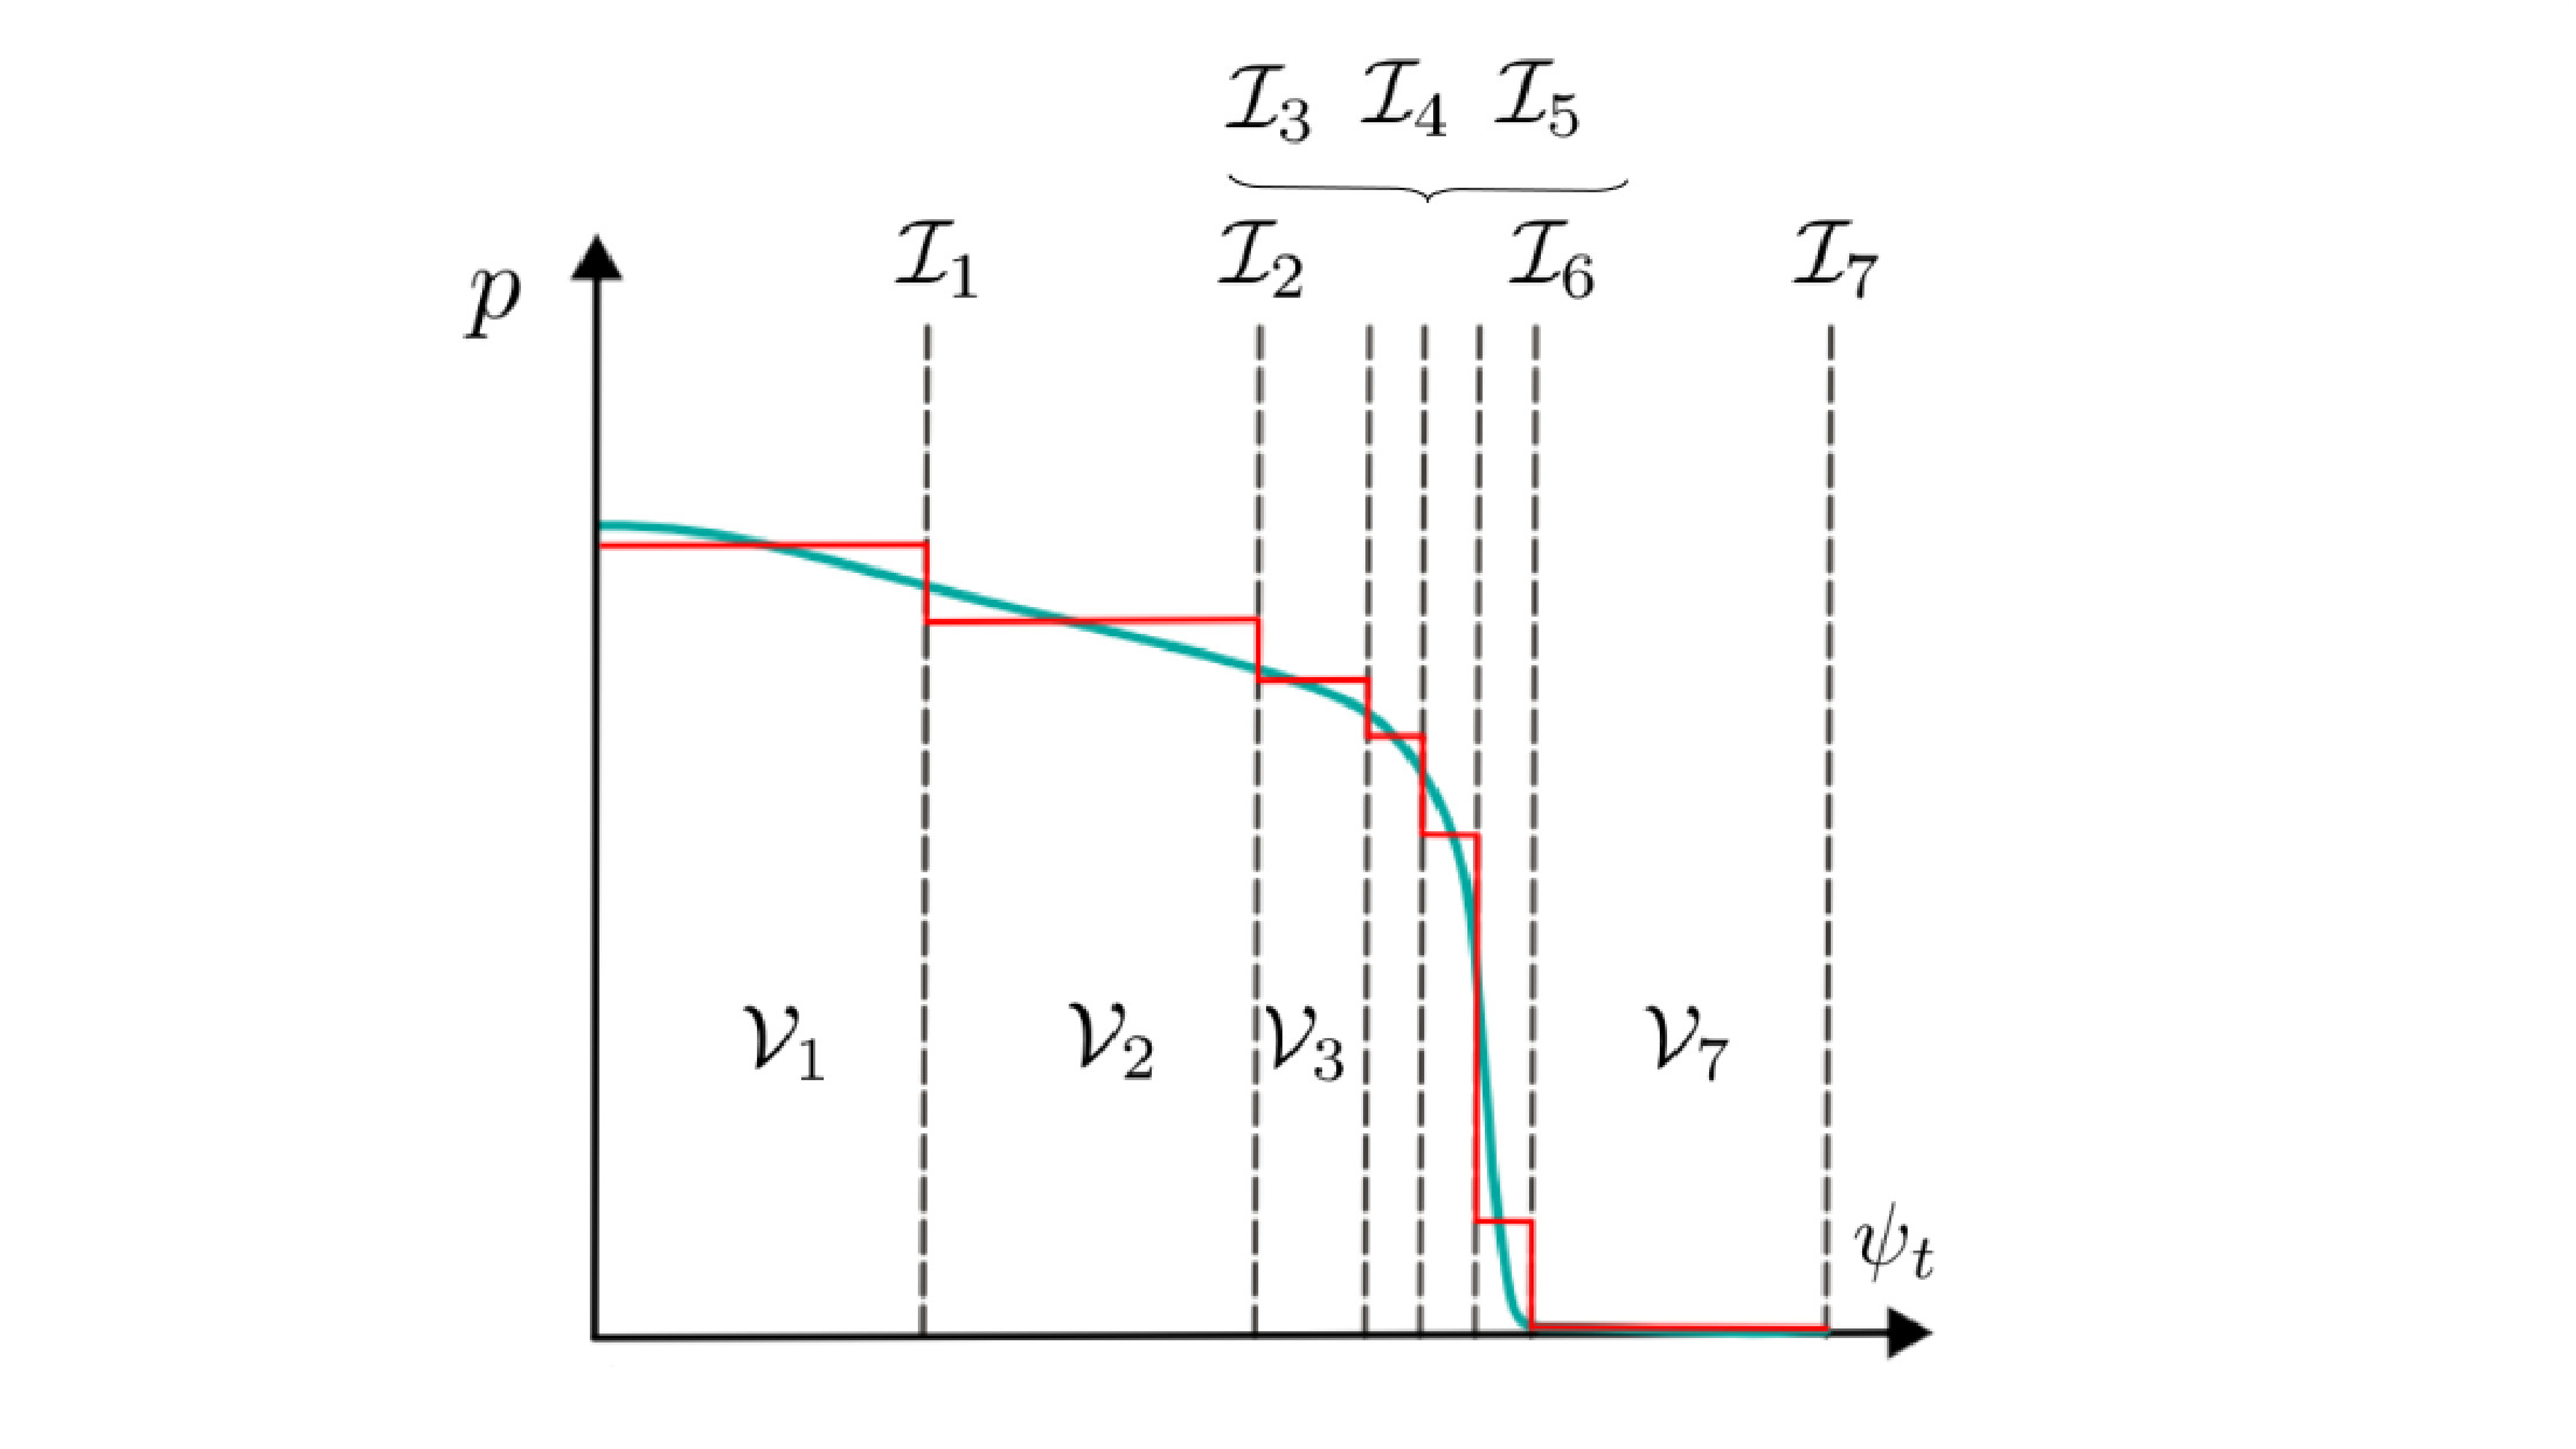
\includegraphics[width=\linewidth]{main/Figures_CurrentConstraint/ABaillod_fig2.pdf}
    \caption{Sketch of a pressure profile as a function of the toroidal flux. Blue: continuous pressure profile obtained via experiment or analytical model. Red: SPEC discretized pressure profile. Black dashed lines: volume interfaces.}
    \label{fig:sketch_pressure}
\end{figure}

A proposed representation of these current density profiles in \ac{MRxMHD} is achieved as follows. The \ac{ECCD} current is an externally driven, parallel current and is thus represented as a volume current since it flows parallel to the field lines; on the other hand, the bootstrap current is a pressure-driven, self-generated current and is represented as a surface current, since it is localized at the pressure gradients. Volume currents are obtained by integrating the externally driven current density in each volume (Figure \ref{fig:sketch_eccd}), which is simply given by the difference

\begin{figure}
    \centering
    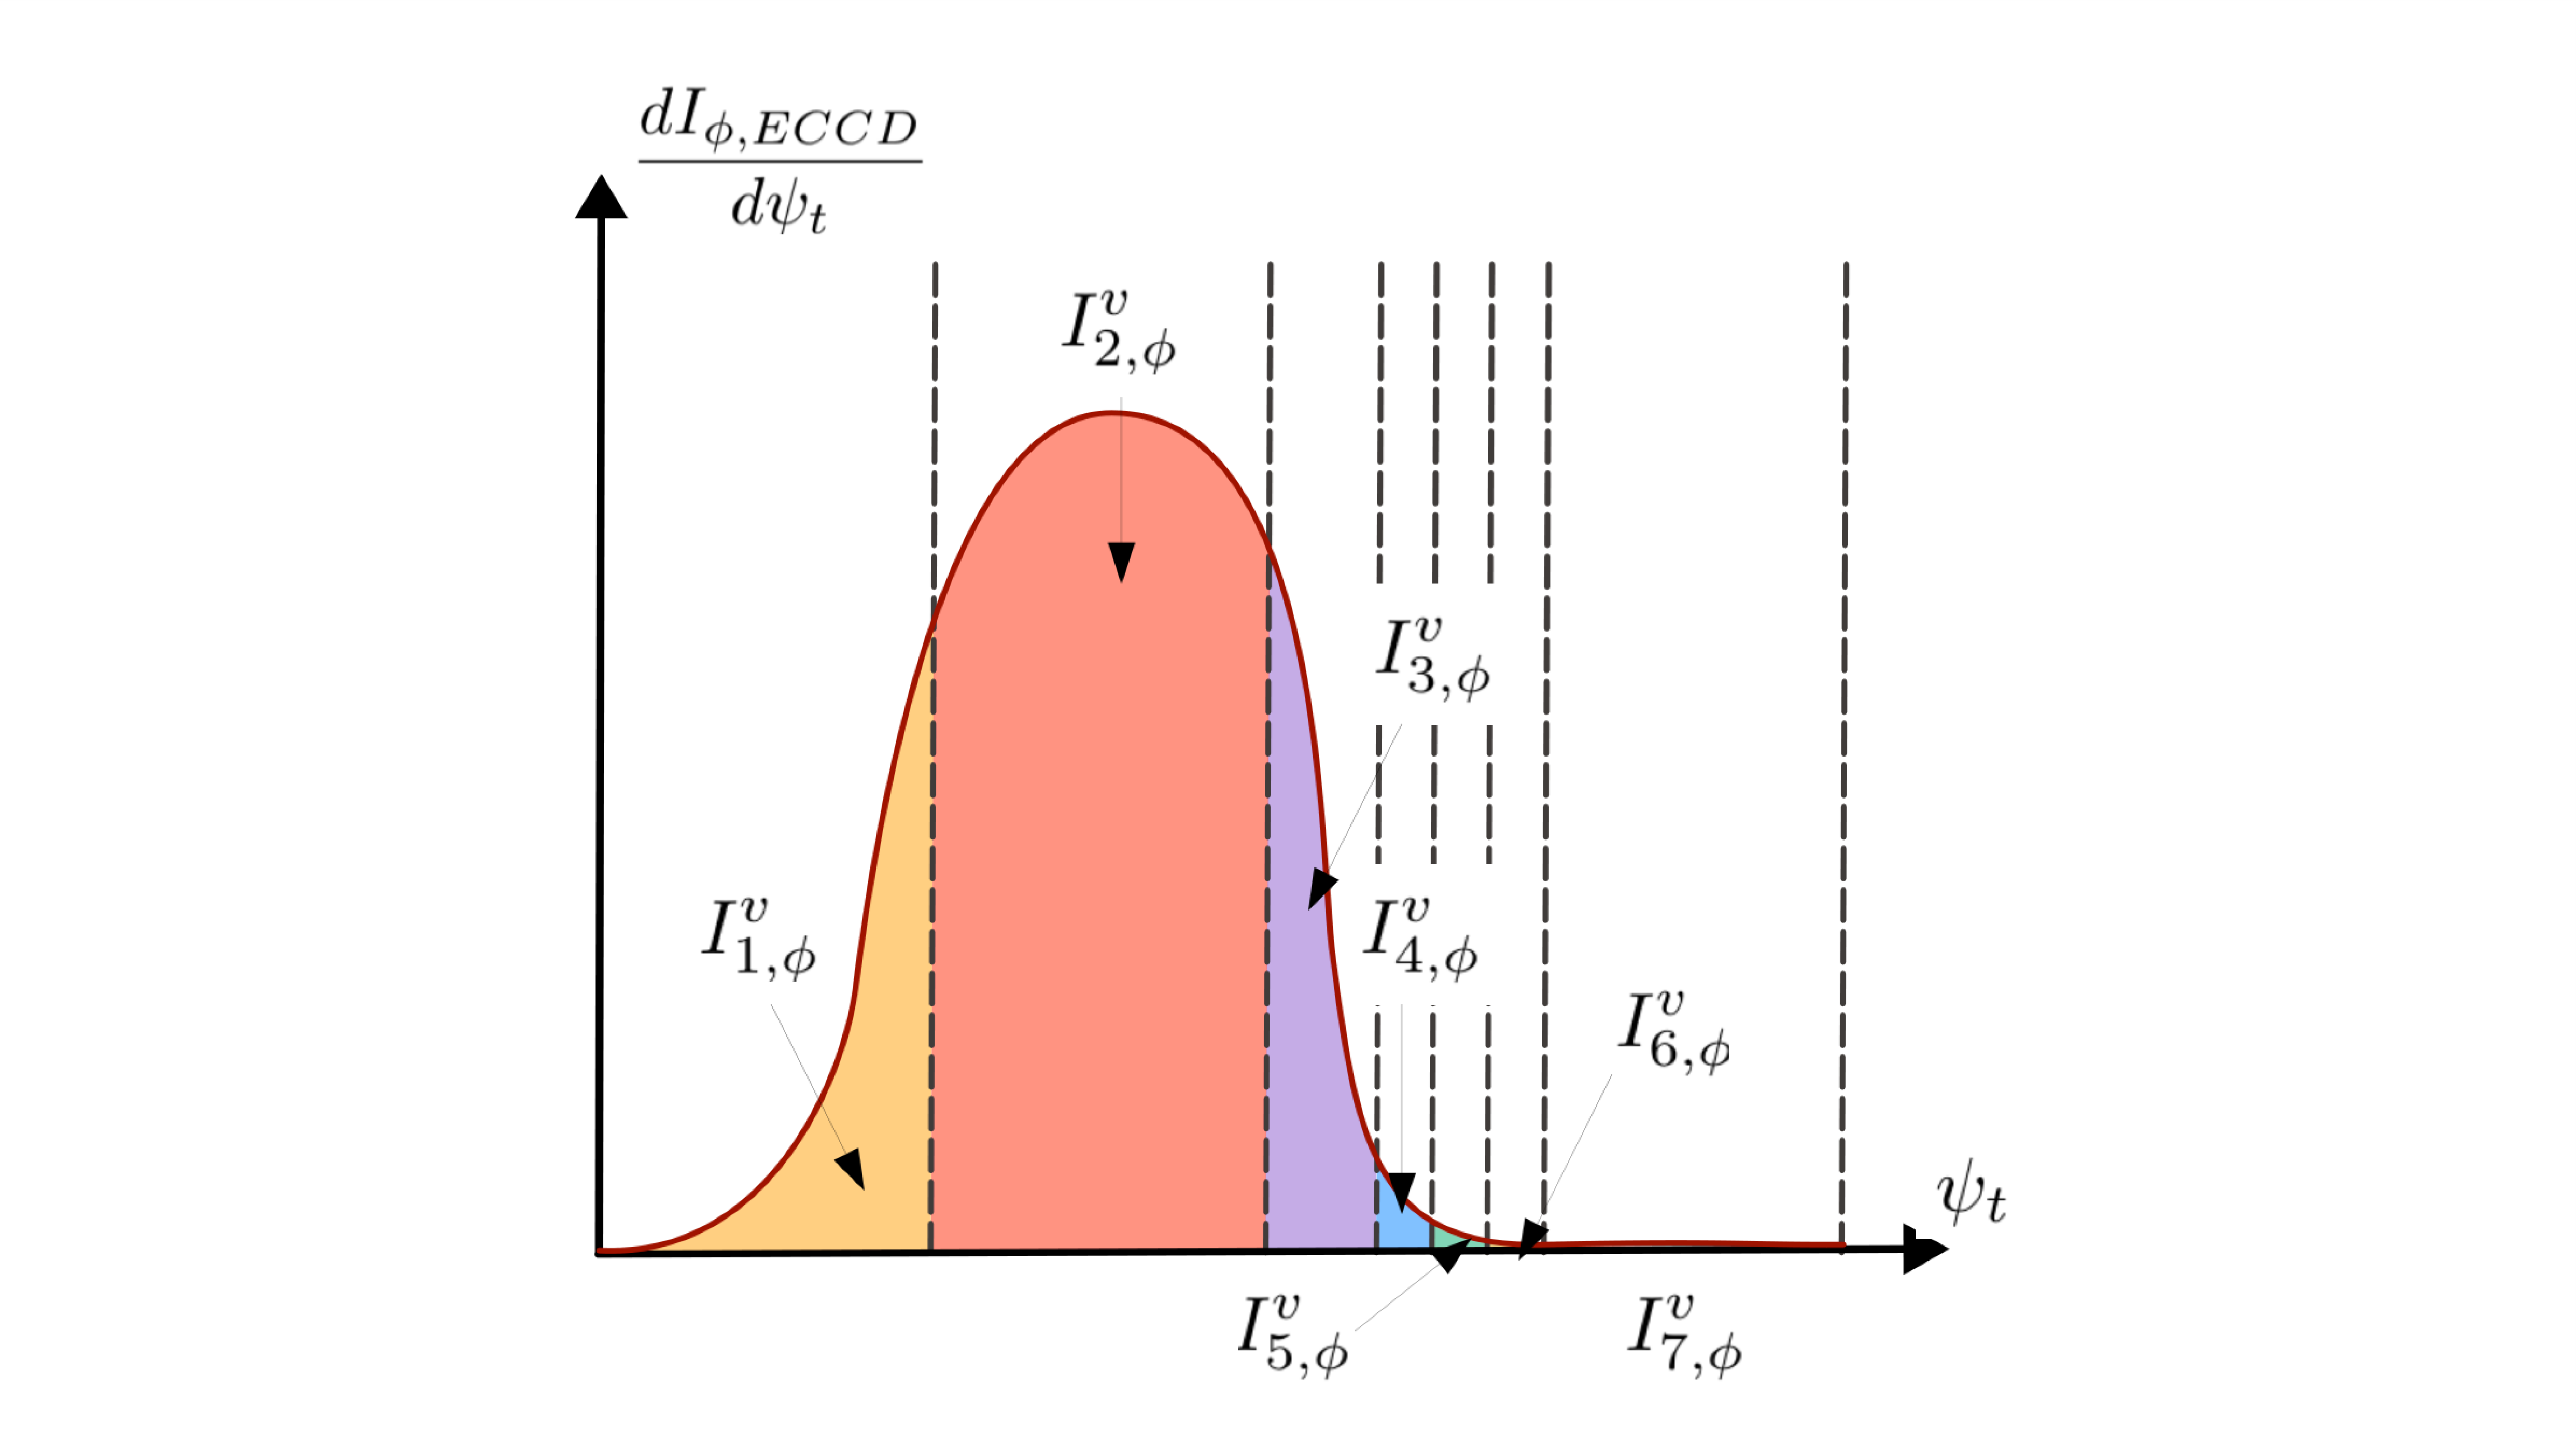
\includegraphics[width=\linewidth]{main/Figures_CurrentConstraint/ABaillod_fig3.pdf}
    \caption{Sketch of externally driven current density (red curve). Colored area correspond to the \ac{MRxMHD} volume current. Black dashed lines represent volume interfaces.}
    \label{fig:sketch_eccd}
\end{figure}


\begin{equation}
    I^v_{l,\phi} = I_{\phi,ECCD}(\psi_{t,l}) - I_{\phi,ECCD}(\psi_{t,l-1}), \label{eq.rep_volume_current}
\end{equation}
and the surface currents are obtained by integrating the pressure driven current density around each interface (Figure \ref{fig:sketch_bootstrap}), which is expressed as

\begin{equation}
    I^s_{l,\phi} = I_{\phi,BS}(\psi_{l,out}) - I_{\phi,BS}(\psi_{l,in}), \label{eq.rep_surface_current}
\end{equation}
with

\begin{align}
    \psi_{l,in} &= \begin{cases}
    0 & \text{if } l=1\\
    \frac{\psi_{t,l-1} + \psi_{t,l}}{2} & \text{otherwise}
    \end{cases}\label{eq.surf_disc1} \\
    \psi_{l,out} &= \begin{cases}
    \psi_{a} & \text{if } l=N_{vol}-1\\
    \frac{\psi_{t,l} + \psi_{t,l+1}}{2} & \text{otherwise}
    \end{cases},\label{eq.surf_disc2}
\end{align}
with $\psi_{a}$ the total toroidal magnetic flux enclosed by the plasma. In Eqs.(\ref{eq.surf_disc1})-(\ref{eq.surf_disc2}), care has been taken for the first and last interfaces, where the surface of integration has been extended to include the current density from the magnetic axis and up to the plasma boundary. Note that this difference in the definition of the first and last surface currents vanishes as the number of volumes $N_{vol}$ is increased. Eqs.(\ref{eq.rep_volume_current})-(\ref{eq.surf_disc2}) are only one possible discretization of the continuous current profiles, proposed by the authors for illustration. Advantages of this particular representation are (1) that the total toroidal current is always preserved and (2) that the currents are approximately localized at the same location in the discretized than in the continuous case. The following sections do not depend on the particular choice of discretization of the currents.


\begin{figure}
    \centering
    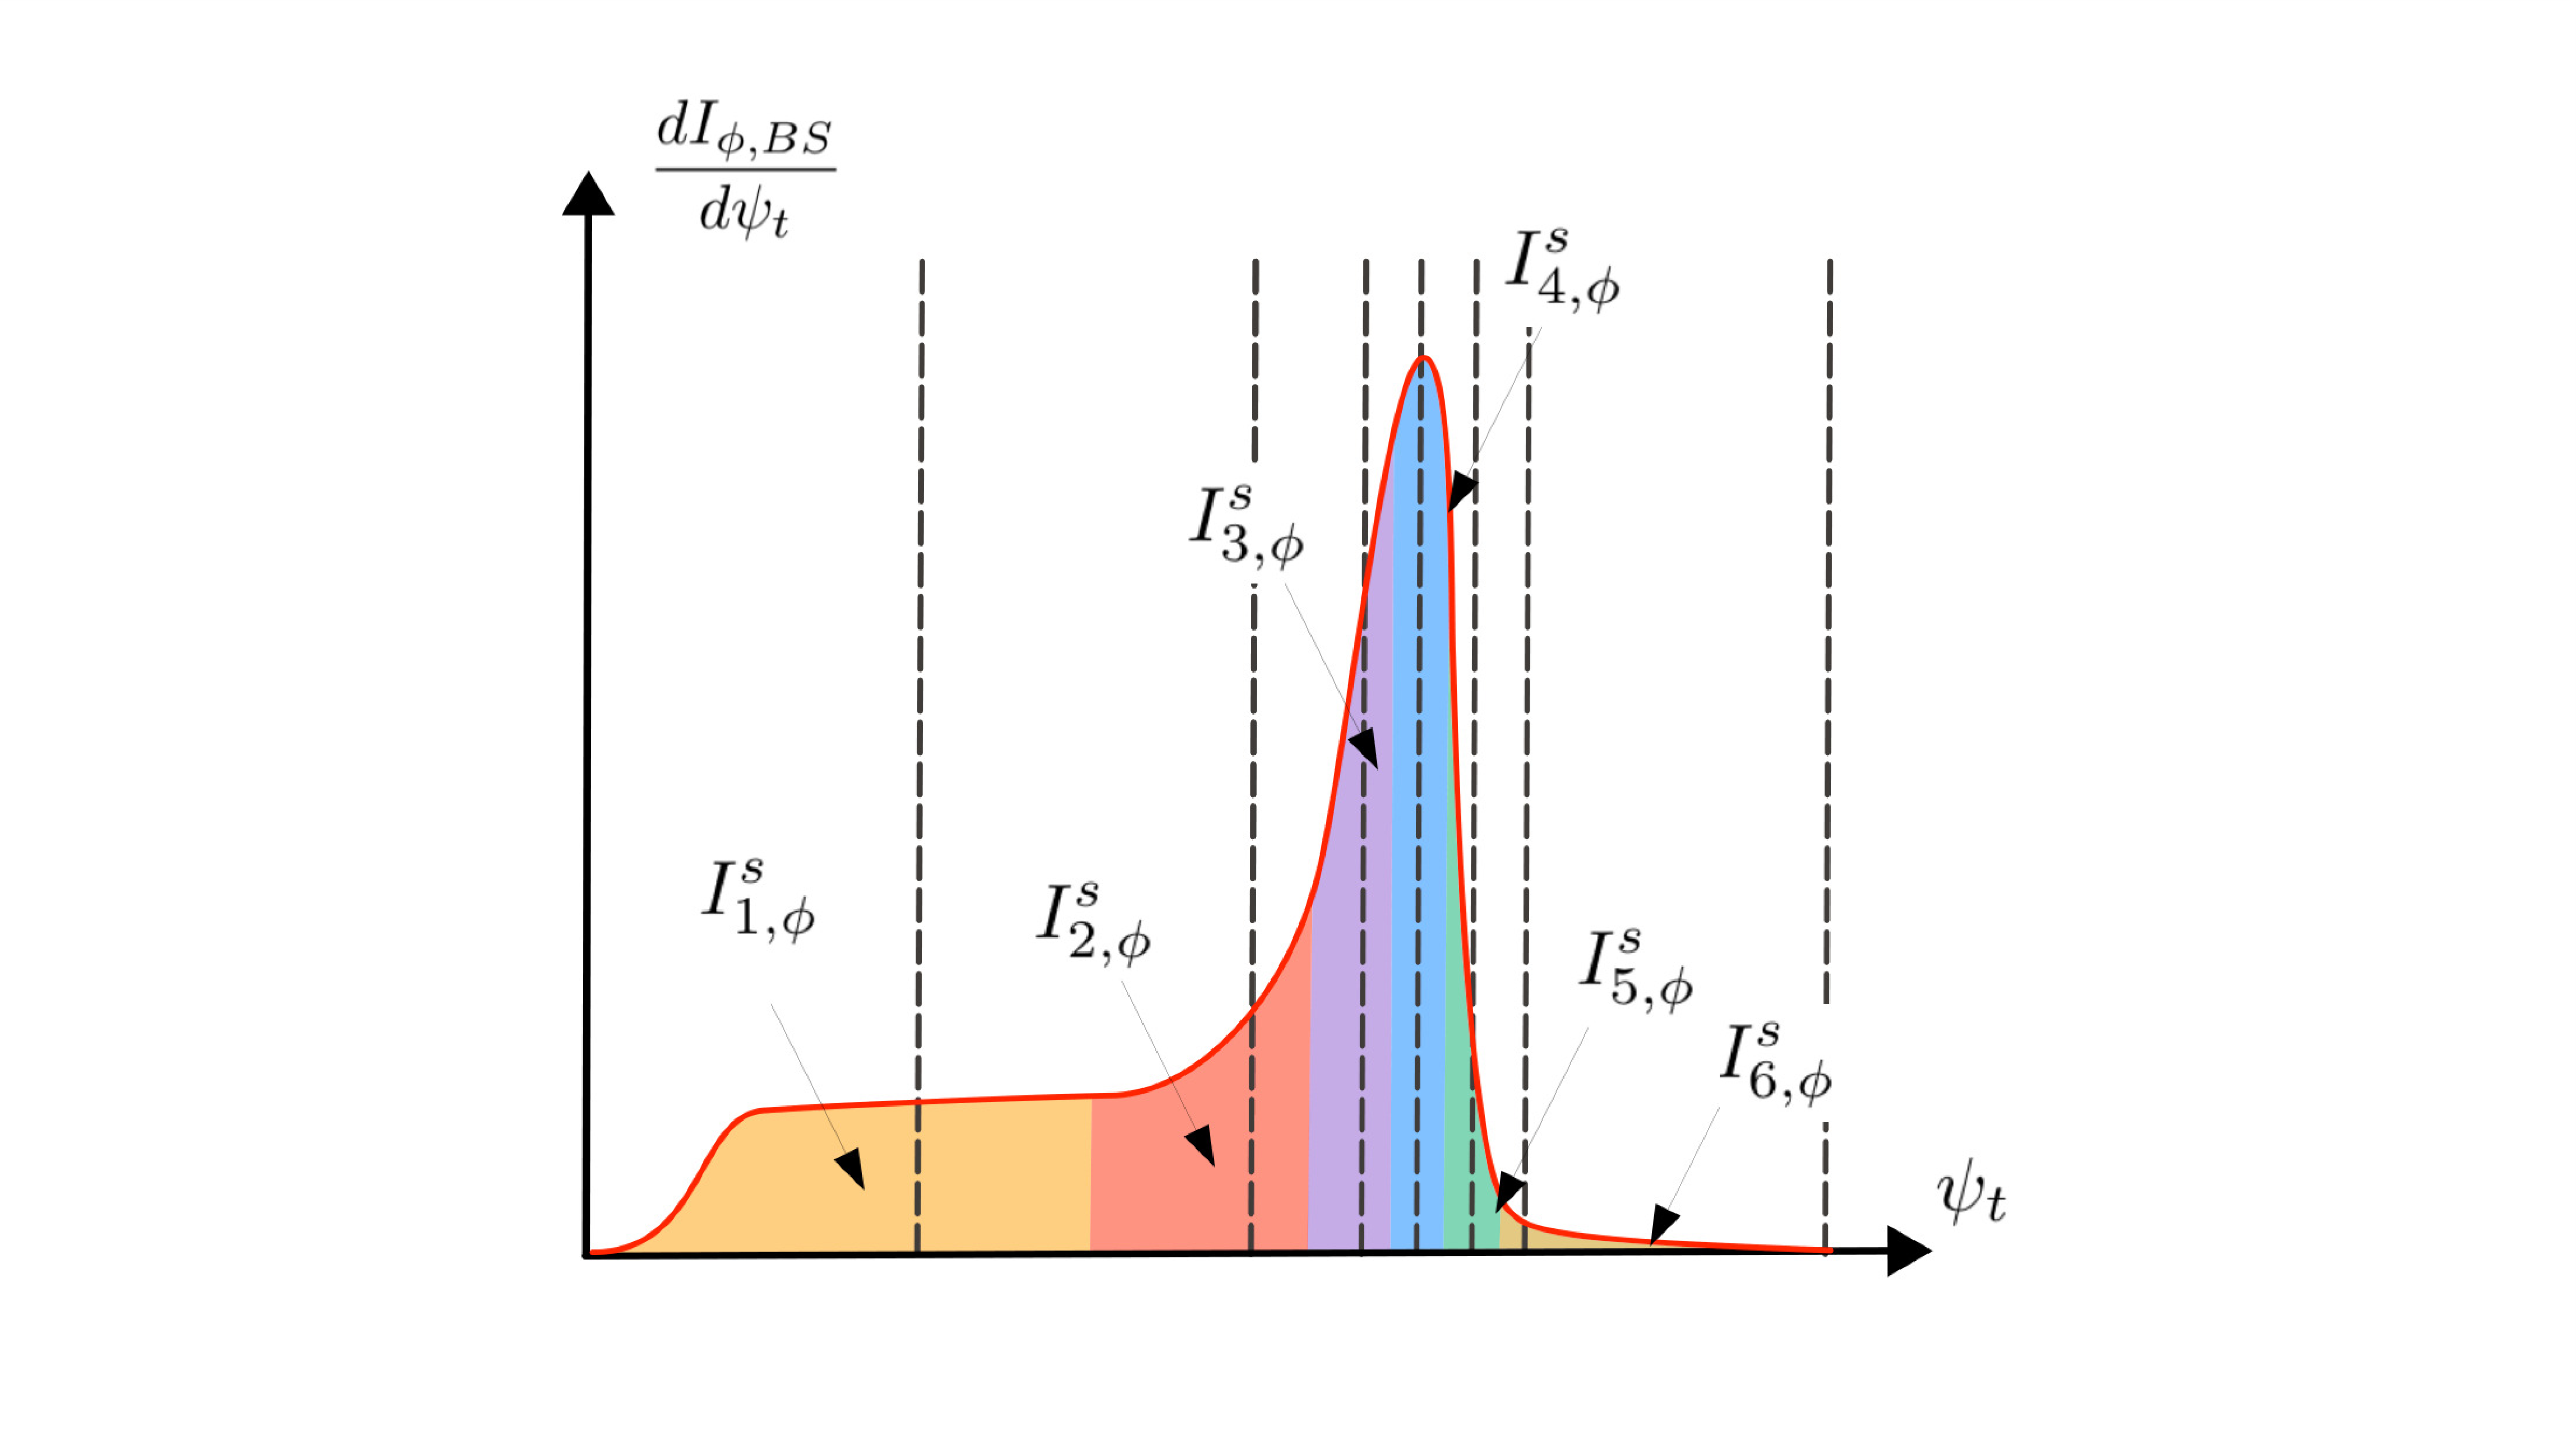
\includegraphics[width=\linewidth]{main/Figures_CurrentConstraint/ABaillod_fig4.pdf}
    \caption{Sketch of pressure driven current density. Colored area correspond to the \ac{MRxMHD} surface current. Black dashed lines represent volume interfaces.}
    \label{fig:sketch_bootstrap}
\end{figure}

\section{Implementation of the current constraint in \ac{SPEC}} \label{sec.spec}

\subsection{The SPEC code}
SPEC can run in three different geometries, namely in slab \citep{Loizu2019},  cylindrical \citep{Loizu2016a} and toroidal geometry \citep{Loizu2016}. The coordinates used to describe position are

\begin{equation}
    \mathbf{x} = \begin{cases}
    \theta\hat{\mathbf{i}} + \phi\hat{\mathbf{j}} + R\hat{\mathbf{k}} \qquad &\text{in slab geometry},\\
    R\cos\theta\hat{\mathbf{i}} + R\sin\theta\hat{\mathbf{j}} + \phi\hat{\mathbf{k}} \qquad &\text{in cylindrical geometry},\\
    R\cos\phi\hat{\mathbf{i}} + R\sin\phi\hat{\mathbf{j}} + Z\hat{\mathbf{k}} \qquad &\text{in toroidal geometry},
    \end{cases}
\end{equation}
where $\{\hat{\mathbf{i}},\hat{\mathbf{j}},\hat{\mathbf{k}}\}$ is the unitary Cartesian basis, $\theta$ is a poloidal angle and $\phi$ is the usual toroidal angle. The geometry of interface $\mathcal{I}_l$, are described by decomposing the coordinates $R$ and $Z$ on a Fourier basis,

\begin{align}
    R_l(\theta,\phi) &= \sum_{m=0}^{M_{pol}}\sum_{n=-N_{tor}}^{N_{tor}}R_{l,m,n} \cos(m\theta-nN_p\phi)\\
    Z_l(\theta,\phi) &= \sum_{m=0}^{M_{pol}}\sum_{n=-N_{tor}}^{N_{tor}}Z_{l,m,n} \sin(m\theta-nN_p\phi),
\end{align}
where $N_p$ is the number of field periods, $M_{pol}$ and $N_{tor}$ are the poloidal and toroidal mode numbers above which Fourier series are truncated, \textit{i.e.} $m=\{0,\ldots,M_{pol}\}$, $n=\{-N_{tor},\ldots,N_{tor}\}$, and stellarator symmetry has been assumed for simplicity. Between interfaces $l$ and $l+1$, coordinates are constructed by linear interpolation of $(R,Z)_l$ and $(R,Z)_{l+1}$ using a radial-like coordinate $s$. Geometrical degrees of freedom are $\{R_{l,m,n}, Z_{l,m,n}\}\equiv\{x_i\}_{i=1,\ldots,N}$, with, \textit{e.g.} in the case of a fixed-boundary, stellarator symmetric equilibrium in toroidal geometry,
\begin{equation}
    N = (N_{vol}-1)\left\{2\left[1+N_{tor} + M_{pol} \left( 2N_{tor} + 1 \right) \right] -1\right\}.
\end{equation}
The magnetic field is represented by the magnetic vector potential, $\mathbf{B}_l=\nabla\times\mathbf{A}_l$, which is described by using a Chebyshev-Fourier basis,

\begin{equation}
    A_{l,i} = \sum_{m,n}\sum_{k=0}^{L_{rad}} A_{l,i,k,m,n} T_k(s)\cos(m\theta-nN_p\phi),
\end{equation}
where $L_{rad}$ is the radial resolution, $T_k$ is the Chebyshev polynomial of order $k$ and $i=\{\theta,\phi\}$. Note that gauge freedom is used to set $A_{l,s}=0\ \forall l$. The coefficients $A_{l,i,k,m,n}$ are the vector potential degrees of freedom, packed in a single array $\mathbf{a}_l$ per volume.

Fixed-boundary \ac{SPEC} can solve the \ac{MRxMHD} system defined by Eqs.(\ref{eq.BeltramiEquation}) and (\ref{eq.force_balance}) for a given plasma boundary geometry, pressure profile $\{p_l\}_{l=1,\ldots,N_{vol}}$ and profiles $\{\psi_{t,l}, \psi_{p,l}, \mu_l\}_{l=1,\ldots,N_{vol}}$. In this case, the Beltrami equation in volume $l$, Eq. (\ref{eq.BeltramiEquation}), can be cast into a linear system
 \begin{equation}
     \mathbf{G}_l\cdot\mathbf{a}_l = \mathbf{C}_l, \label{eq.linearized_beltrami_system}
 \end{equation}
 where $\mathbf{G}_l$ and $\mathbf{C}_l$ are matrices that depend only on the geometrical degrees of freedom  $\{x_i\}_{i=1,\ldots,N}$, and linearly on $\psi_{t,l}$, $\psi_{p,l}$ and $\mu_l$. 
 
 The constrained quantities $\{\mu_l,\psi_{t,l},\psi_{p,l}\}_{l=1,\ldots,N_{vol}}$ can be replaced by other independent triplets such as $\{\psi_{t,l},\ \iotabar_l^+,\  \iotabar_l^-\}_{l=1,\ldots,N_{vol}}$, with $\iotabar_l^\pm$ the rotational transform evaluated on the inner and outer side of interface $\mathcal{I}_l$, respectively. In this case, \ac{SPEC} iterates on $\{\psi_{p,l}, \mu_l\}_{l=1,\ldots,N_{vol}}$ until the solution satisfies the input rotational transform profile. In what follows, this method will be referred to as the \emph{rotational transform constraint}. Finally, \ac{SPEC} uses a Newton method to iterate on $\{x_i\}_{i=1,\ldots,N}$ until the force balance, Eq.(\ref{eq.force_balance}), is satisfied. This is achieved by expanding the force imbalance on a Fourier basis,
 
 \begin{equation}
     \left[\left[p+\frac{B^2}{2\mu_0}\right]\right]_l = \sum_{m=0}^{M_{pol}}\sum_{n=-N_{tor}}^{N_{tor}} F_{l,m,n} \cos(m\theta-nN_p\phi),
 \end{equation}
 and packing the Fourier components $F_{l,m,n}$ in a single array $\mathbf{F}$ of size $N$. Force balance is satisfied once all the Fourier modes $F_{l,m,n}$, herein $\{F_j\}_{j=1,\ldots,N}$, are sufficiently small. Analytical derivatives of $\{F_j\}_{j=1,\ldots,N}$ with respect to $\{x_i\}_{i=1,\ldots,N}$ accelerate substantially the code.
 
 It is worth noting that even though the magnetic helicity is not conserved when \ac{SPEC} iterates on $\{x_i\}_{i=1,\ldots,N}$ to find an equilibrium that matches a given input $\{\psi_{t,l}, \psi_{p,l}, \mu_l\}_{l=1,\ldots,N_{vol}}$ or $\{\psi_{t,l},\ \iotabar_l^+,\  \iotabar_l^-\}_{l=1,\ldots,N_{vol}}$, the final equilibrium satisfies the \ac{MRxMHD} equilibrium equations (Eq.(\ref{eq.BeltramiEquation})-(\ref{eq.force_balance})). There is a magnetic helicity profile $\{K_l\}_{l=1,\ldots,N_{vol}}$ corresponding to this equilibrium which is unknown \textit{a priori}. Thus, the same equilibrium could have been found by minimizing the \ac{MRxMHD} energy functional while keeping the magnetic helicity profile constant if the initial state had the same magnetic helicity profile (bifurcations are not considered in this chapter). This capability is also available in \ac{SPEC}, and details can be found in the literature \citep{Hudson2012,Dennis2013a}.

 Lastly, \ac{SPEC} has been recently extended to allow free-boundary calculations \citep{Hudson2020c}, where the plasma is surrounded by a vacuum region bounded by a computational boundary. The solution in the vacuum region, which is a special instance of a Beltrami field, with $\mu=0$, is determined by a different set of scalars, namely the total poloidal current passing through the torus hole, $I_{coil}$, and the total toroidal plasma current, $I_{pl}$. Using Ampere's law, these currents can be written as
 
 \begin{align}
 \mu_0 I_{coil} &= 2\pi\tilde{B}^+_{V,\phi}\\
 \mu_0 I_{pl} &= 2\pi\tilde{B}^-_{V,\theta},
 \end{align}
 with $\tilde{B}^+_{V,\phi}$ the $m=n=0$ Fourier mode of the covariant toroidal magnetic field on the computational boundary and $\tilde{B}^-_{V,\theta}$ the $m=n=0$ Fourier mode of the covariant poloidal magnetic field on the outer side of the plasma boundary. Additionally, the computational boundary is not necessarily a flux surface, thus $\mathbf{B}_V\cdot\hat{\mathbf{n}}_c \neq 0$ with $\mathbf{B}_V$ the magnetic field in the vacuum region and $\hat{\mathbf{n}}_c$ a unit vector normal to the computational boundary. The solution satisfying the constraints $I_{coil}$ and $I_{pl}$ is obtained by iteration over the poloidal and toroidal fluxes $\{\psi_{p,V},\psi_{t,V}\}$ in the vacuum volume.
 
 \subsection{Constraining the toroidal current profiles in \ac{SPEC}}
 
\ac{SPEC} has been extended to allow the triplet $\{\psi_{t,l}, I^v_{l,\phi}, I^s_{l,\phi}\}_{l=1,\ldots,N_{vol}}$ as a constraint, herein \textit{current constraint}. In the case of the rotational transform constraint, \ac{SPEC} finds the solution to the linear system (\ref{eq.BeltramiEquation}) volume by volume and iterates on $\{\mu_l, \psi_{p,l}\}$ until the field has the desired rotational transform at the volume interfaces. In the case of the current constraint, the constants $\{\mu_l\}_{l=1,\ldots,N_{vol}}$ are determined using Eq.(\ref{eq.volume_current}), without the need for iterations, and this directly constrains the value of volume currents $\{I^v_{l,\phi}\}_{l=1,\ldots,N_{vol}}$.

Regarding the poloidal fluxes, it can be shown  (Appendix \ref{appA1}) that the surface currents depend linearly on the poloidal fluxes, \textit{i.e.} 

\begin{equation}
\mathbf{I}^s=\mathbf{M}\bm{\psi}_p+\mathbf{Q}\label{eq.complicado},    
\end{equation}
where $\mathbf{I}^s$ and $\bm{\psi}_p$ are arrays containing all $\{I^s_l\}_{l=1,\ldots,N_{vol}-1}$ and all $\{\psi_{p,l}\}_{l=2,\ldots,N_{vol}}$ respectively, and the matrix $\mathbf{M}$ and the  array $\mathbf{Q}$ depend only on the geometry of the interfaces $\{x_i\}_{i=1,\ldots,N}$. In this section, we consider the geometry, toroidal fluxes and the constants $\{\mu_l\}_{l=1,\ldots,N_{vol}}$ to be fixed and seek how the poloidal flux profile $\bm{\psi}_p$ has to be constrained in order to obtain a surface current profile matching the input profile $\mathbf{I}^s$.

The unknown $\mathbf{Q}$ is eliminated by subtracting Eq.(\ref{eq.complicado}) evaluated at two different values of $\bm{\psi}_p$, \textit{i.e.} evaluated once at $\overbar{\bm{\psi_p}}$ and once at $\bm{\psi}_p$,
\begin{equation}
    \mathbf{M} (\overbar{\bm{\psi}_p} - \bm{\psi}_p) = \overbar{\bm{I}^{s}} - \bm{I}^{s}, \label{eq.psip_diff}
\end{equation}
where $\overbar{\bm{\psi}_p}$ is an arbitrary choice of poloidal fluxes, and $\overbar{\bm{I}^s}$ is the surface current profile calculated from the Beltrami fields $\{\overbar{\mathbf{a}_l}\}_{l=1,\ldots,N_{vol}}$ obtained when the poloidal fluxes are constrained to the values $\overbar{\bm{\psi}_p}$.

The matrix $\mathbf{M}$ is evaluated by taking the derivatives of Eq.(\ref{eq.complicado}) with respect to the poloidal fluxes, \textit{i.e.}

\begin{equation}
    M_{ij} = \frac{\partial I^s_{i,\phi}}{\partial \psi_{p,j}},\label{eq.coef_M}
\end{equation}
which leads to the following bi-diagonal matrix

\begin{equation}
    \mathbf{M} = \frac{2\pi}{\mu_0} \begin{bmatrix}\dfrac{\partial \tilde{B}^-_{\theta,2}}{\partial{\psi_{p,2}}} & 0 & \cdots & \cdots  & 0 \\
    -\dfrac{\partial \tilde{B}^+_{\theta,2}}{\partial{\psi_{p,2}}} & \dfrac{\partial \tilde{B}^-_{\theta,3}}{\partial{\psi_{p,3}}} & 0  & \cdots & 0\\
    0 & -\dfrac{\partial \tilde{B}^+_{\theta,3}}{\partial{\psi_{p,3}}} & \dfrac{\partial \tilde{B}^-_{\theta,4}}{\partial{\psi_{p,4}}} & 0  & 0 \\
    \vdots & \ddots & \ddots  & \ddots & 0\\
    0 \cdots  & \cdots & 0 & -\dfrac{\partial \tilde{B}^+_{\theta,N_{vol}-1}}{\partial{\psi_{p,N_{vol}-1}}} & \dfrac{\partial \tilde{B}^-_{\theta,N_{vol}}}{\partial{\psi_{p,N_{vol}}}}\end{bmatrix}.\label{eq.matrix_M}
\end{equation}
Derivatives of $\tilde{B}^\pm_{\theta,l}$ with respect to the poloidal flux can be easily obtained by applying matrix perturbation theory on the linear system (\ref{eq.linearized_beltrami_system}) \citep{Hudson2012},

\begin{equation}
    \mathbf{G}_l \cdot \left[\frac{\partial}{\partial\psi_{p,l}}\mathbf{a}_l\right] = - \left[\frac{\partial}{\partial\psi_{p,l}}\mathbf{G}_l\right] \cdot \mathbf{a}_l + \frac{\partial}{\partial\psi_{p,l}}\mathbf{C}_l.\label{eq.perturbed_matrix}
\end{equation}

Due to the linear nature of Eq.(\ref{eq.complicado}), the coefficients of the matrix $\mathbf{M}$, \textit{i.e.} Eq.(\ref{eq.coef_M}), are independent of $\bm{\psi}_p$ and thus can be evaluated once at any arbitrary value of $\bm{\psi}_p$. We thus conveniently evaluate them at $\overbar{\bm{\psi}_p}$. Equation (\ref{eq.psip_diff}) is then solved to obtain the poloidal flux profile $\bm{\psi}_p$. 

Finally, instead of solving a second time the Beltrami equation, Eq.(\ref{eq.BeltramiEquation}), at $\bm{\psi}_p$, we take advantage of the linear dependence of $\mathbf{a}$ on $\bm{\psi}_p$, Eq.(\ref{eq.linearized_beltrami_system}), and solve  

\begin{equation}
    A_{l,i} = \overbar{A_{l,i}} - \frac{\partial {A_{l,i}}}{\partial {\psi_{p,l}}} (\overbar{\psi_{p,l}} - \psi_{p,l}),\label{eq.NewtonStep_Solution}
\end{equation}
where $\overbar{A_{l,i}}$ is one element of $\overbar{\bm{a}_l}$. The algorithm flow is summarized in Figure \ref{fig.algo_current_constraint}.

\begin{figure}
    \centering
    \begin{tikzpicture}
    \tikzstyle{MyAlgoStep}=[draw,text width=3.5cm,text centered,rounded corners=3pt]
    \tikzstyle{MyBigAlgoStep}=[draw, text width=8cm,text centered,rounded corners=3pt]
    \node[MyBigAlgoStep] (init) at (0,5) {
    	1) Set the toroidal flux profile $\{\psi_{t,l}\}_{l=1,\ldots,N_{vol}}$ from input and the constants $\{\mu_{t,l}\}_{l=1,\ldots,N_{vol}}$ using the volume current profile and Eq.(\ref{eq.volume_current})
    };
    \node[draw, thick, dashed] (O) at (0,.7) {
    \begin{minipage}[t][5.8cm]{.95\textwidth}
    \centering
    2) Solve Beltrami equations consistently with the input surface current constraint
    \end{minipage}
    };
    \node[MyAlgoStep] (A) at (-4.5,1.5) {2.1) Chose an arbitrary $\overbar{\bm{\psi_p}}$};
    \node[MyAlgoStep] (B) at (0,1.5) {2.2) Solve Beltrami equation (\ref{eq.BeltramiEquation}) by constraining the poloidal fluxes to the values $\overbar{\bm{\psi_p}}$ to get $\overbar{\mathbf{a}_l}$};
    \node[MyAlgoStep] (C) at (4.5,1.5) {2.3) Solve perturbed matrix equation (\ref{eq.perturbed_matrix}) to get $\dfrac{\partial \overbar{\mathbf{a}_l} }{\partial \psi_{p,l}}$};
    \node[MyAlgoStep] (D) at (4.5,-1) {2.4) Build matrix $\mathbf{M}$ by constructing $\dfrac{\partial \tilde{B}^\pm_{\theta,l}}{\partial \psi_p}$ from $\dfrac{\partial \overbar{\mathbf{a}_l} }{\partial \psi_{p,l}}$};
    \node[MyAlgoStep] (E) at (0,-1) {2.5) Solve equation (\ref{eq.psip_diff}) and get $\bm{\psi_p}$};
    \node[MyAlgoStep] (F) at (-4.5,-1) {2.6) Find $\mathbf{a}$ by solving Eq.(\ref{eq.NewtonStep_Solution})};
    \draw[->,>=latex] (init) -- (O); 
    \draw[->,>=latex] (A) -- (B);
    \draw[->,>=latex] (B) -- (C);
    \draw[->,>=latex] (C) -- (D);
    \draw[->,>=latex] (D) -- (E);
    \draw[->,>=latex] (E) -- (F);
    \end{tikzpicture}
    \caption{Flow of the algorithm used to constrain the net toroidal current profiles for a given toroidal flux profile and geometry.}
    \label{fig.algo_current_constraint}
\end{figure}

In the case of a free-boundary computation, the toroidal flux in the vacuum region is varied to satisfy the poloidal linking current $I_{coil}$. This slightly modifies the linear system (\ref{eq.psip_diff}). Details can be found in Appendix \ref{appA}.

Constraining the toroidal current profile takes away the control of other profiles such as the rotational transform or the magnetic helicity. However, as for the case of the rotational transform constraint, the equilibrium can be accessed by a relaxation process at constant magnetic helicity if the final magnetic helicity is known \textit{a priori}. The \ac{MRxMHD} equations are thus still satisfied by an equilibrium obtained by constraining the toroidal current profiles. 

\subsection{Force gradient}

The Newton algorithm used in SPEC to iterate on the interfaces geometry uses analytic derivatives, which is faster than finite differentiation. To keep good performance while using the current constraint, derivatives of the force Fourier coefficients, $\{F_j\}_{j=1,\ldots,N}$, with respect to the interfaces degrees of freedom, $\{x_i\}_{i=\{1,\ldots,N\}}$, at constant $\{\psi_{t,l}, I^v_{l,\phi},\ I^s_{l,\phi}\}_{l=1,\ldots,N_{vol}}$ are provided. Derivatives are first evaluated in real space and then Fourier-transformed. Using the chain rule,
\begin{align}
    \frac{d}{d x_i}\left[\left[p + \frac{B^2}{2\mu_0}\right]\right]_l &= \frac{1}{\mu_0}\left( B^-_{l+1}\frac{d B^-_{l+1}}{d x_i} - B^+_l \frac{d B^+_{l}}{d x_i}\right)\\ \label{eq.force_gradient}
    \frac{d B^{\pm}_l}{d x_i} &= \frac{\partial B^\pm_l}{\partial x_i} + \frac{\partial B^\pm_l}{\partial \psi_{p,l}}\frac{d \psi_{p,l}}{d x_i} + \frac{\partial B^\pm_l}{\partial \mu_l}\frac{d\mu_l}{d x_i}+ \frac{\partial B^\pm_l}{\partial \psi_{t,l}}\frac{d\psi_{t,l}}{d x_i}
\end{align}
where $B^-_l$, $B^+_l$ are the magnetic field strength on the inner and outer side of volume $l$, respectively, and the pressure, $p_l$, is considered constant in each volume with respect to variations in the geometry, $\mu_l$ and $\psi_{p,l}$. Note that all derivatives are taken at constant toroidal flux, volume current and surface current. Enforcing $ d\psi_{t,l} / dx_i=0$ and $d I^v_{l,\phi} / dx_i=0$ leads to $d \mu_l/dx_i=0$ using Eq.(\ref{eq.volume_current}). The surface current constraint, $d I^s_{l,\phi}/dx_i=0$, leads to a system of coupled equations using Eq.(\ref{eq.surf_current}),
     
\begin{equation}
    \frac{\partial \tilde{B}^-_{l+1,\theta}}{\partial x_i} + \frac{\partial \tilde{B}^-_{l+1,\theta}}{\partial \psi_{p,l+1}} \frac{\partial\psi_{p,l+1}}{\partial x_i} - \frac{\partial \tilde{B}^+_{l,\theta}}{\partial x_i} - \frac{\partial \tilde{B}^+_{l,\theta}}{\partial \psi_{p,l}}\frac{\partial\psi_{p,l}}{\partial x_i} = 0, \label{eq.Isurface_derivative}
\end{equation}
which can be written as a linear system using the matrix $\mathbf{M}$ defined in Eq.(\ref{eq.matrix_M}),
     
\begin{equation}
    \mathbf{M} \cdot  \begin{bmatrix}
    \dfrac{d\psi_{p,2}}{dx_i}\\
    \vdots\\
    \dfrac{d\psi_{p,N_{vol}}}{dx_i}
    \end{bmatrix} = \frac{2\pi}{\mu_0}\begin{bmatrix}
    \dfrac{\partial \tilde{B}^+_{\theta,1}}{\partial x_i} - \dfrac{\partial \tilde{B}^-_{\theta,2}}{\partial x_i} \\
    \vdots \\
    \dfrac{\partial \tilde{B}^+_{\theta,N_{vol}-1} } {\partial x_i} - \dfrac{\partial \tilde{B}^-_{\theta,N_{vol}}}{\partial x_i}
    \end{bmatrix}.\label{eq.linear_system}
\end{equation}
Derivatives of $\tilde{B}_{\theta,l}$ with respect to $\psi_{p,l}$ and $x_i$ can be obtained by applying matrix perturbation theory to the Beltrami system (\ref{eq.linearized_beltrami_system}). The solution of Eq.(\ref{eq.linear_system}), together with Eq.(\ref{eq.force_gradient}) provides the required derivatives of the force with respect to the geometry. Derivatives of the Fourier components of the force, $dF_j/dx_i$, are obtained by taking the Fourier transform of equation (\ref{eq.force_gradient}) and are packed in a matrix $\nabla F$ of size $N^2$, henceforth named \textit{force gradient}. Appendix \ref{appA} provides details on the free-boundary case. 

\subsection{Implementation details and parallelization}
The new current constraint has been parallelized with \ac{MPI} in a similar fashion to the other constraints. Each volume is associated to one \ac{CPU}; since the solution to the Beltrami equation (\ref{eq.BeltramiEquation}) in a volume is independent from other volumes, each \ac{CPU} can solve the linear system (\ref{eq.linearized_beltrami_system}) in parallel. Finally, the master \ac{CPU} gathers all required derivatives to construct the matrix $\mathbf{M}$ and solves the linear system (\ref{eq.psip_diff}), before broadcasting the values of $\{\psi_{p,l}\}_{l=2,\ldots,N_{vol}}$ and $\{\mathbf{a}_l\}_{l=1,\ldots,N_{vol}}$ to all \acp{CPU}.

Regarding communications, we reduced them to a minimum. The global toroidal current constraint is computed using Eq.(\ref{eq.surf_current}), which only depends on the first even Fourier coefficient of $B_\theta$ in each volumes. We thus compute locally (by each \ac{MPI} task) these coefficients before sending them to the master task. This requires the communication of $2(N_{vol}-1)$ doubles. All communications are implemented using basic \ac{MPI} point-to-point communications, though a gathering communication could be more efficient. The master task then solves Eqs.(\ref{eq.psip_diff}) and (\ref{eq.NewtonStep_Solution}) and broadcasts the elements $\overbar{\bm{a}_l}$ and $\overbar{\bm{\psi}_p}$. We don't expect a communication bottleneck due to the reasonably low amount of communications. 

%\subsubsection{Code complexity}
%\label{sec:theoretical_complexity}
%The theoretical complexity of \ac{SPEC} depends on the number of volumes $N_{vol}$ and the radial, poloidal and toroidal resolution $L_{rad}$, $M_{pol}$ and $N_{tor}$ respectively. One of the most time consuming part is the computation of the geometry-dependent matrices. These matrices have $L_{rad}^2\cdot M_{pol}^2\cdot N_{tor}^2$ elements and are computed in each volume. The time spent computing these matrices grows as
%
%\begin{equation}
%	\mathcal{O}_{matrices} \sim \mathcal{O}(N_{vol} L_{rad}^2 M_{pol}^2 N_{tor}^2).
%\end{equation}
%These matrices are evaluated each time the geometry is changed, which depends on the sought equilibrium. Another time consuming part of the calculation is the force gradient evaluation, where Eq.(\ref{eq.linear_system}) has to be solved for each geometrical degree of freedom $x_i$. The number of degrees of freedom scales as $\mathcal{O}(N_{vol}M_{pol}N_{tor})$.
%
%
%SPEC theoretical complexity is thus
%
%\begin{equation}
%	\mathcal{O}_{SPEC} = \mathcal{O}(N_{vol} L_{rad}^2M_{pol}^2N_{tor}^2).
%\end{equation}
%We thus expect a cubic relation between the time to solution and the number of volumes. We can already see that SPEC won't scale well with the number of volumes - doubling the number of volume would require eight time more MPI tasks. However, having more MPI tasks than the number of volume is pointless: the parallelization topology forces us to use a maximum of $N_{vol}$ MPI tasks. Others would be unused.
%
%However we can study how the code will scale with the parameter $N_{scale}\equiv L_{rad}^2M_{pol}^3N_{tor}^3$. Since the number of communications does not increase with $N_{scale}$, we expect no negative effects on the parallelization efficiency.

 
\section{Verification of the current constraint} \label{sec.verification}
 
 In this section we present a rigorous verification of the new capability of \ac{SPEC} against analytical solutions in a screw pinch geometry and against a reference \ac{SPEC} solution obtained with the rotational transform constraint in a classical stellarator geometry. All results presented in this paper were obtained with \ac{SPEC} version 2.10.
 
 \subsection{Verification in cylindrical geometry}
 
 We consider a fixed-boundary screw pinch \ac{MRxMHD} equilibrium that only depends on the radius $R$ and whose solutions can be written analytically (Appendix \ref{appB}). We choose a set of somewhat arbitrary input parameters, \textit{i.e.} a cylinder of minor radius $a=1$ and length $L=2\pi$, $N_{vol}=3$, $p_l=0$ $\forall l\in\{1,2,3\}$, $\bm{\psi}_t = \{1/9, 4/9, 1\}$Tm${}^2$, $\mu_0\mathbf{I}^v=\{0.2,0.2,0.4\}$Tm and $\mu_0\mathbf{I}^s=\{-0.4,0.5\}$Tm, which uniquely define the analytical solution. \ac{SPEC} is then run with the same input parameters and the solutions are compared (Figure \ref{fig:SP_constraint_verification}). Very good agreement between the analytical solution and the \ac{SPEC} solution is obtained. Note that by constraining the toroidal current profiles, we lose control on the rotational transform profile, since only two profiles can be constrained in addition to the pressure profile. Hence discontinuities in the magnetic field components arise at the volume interfaces, even when there is no pressure, unless the input parameters are carefully selected.
 
 \begin{figure}
     \centering
     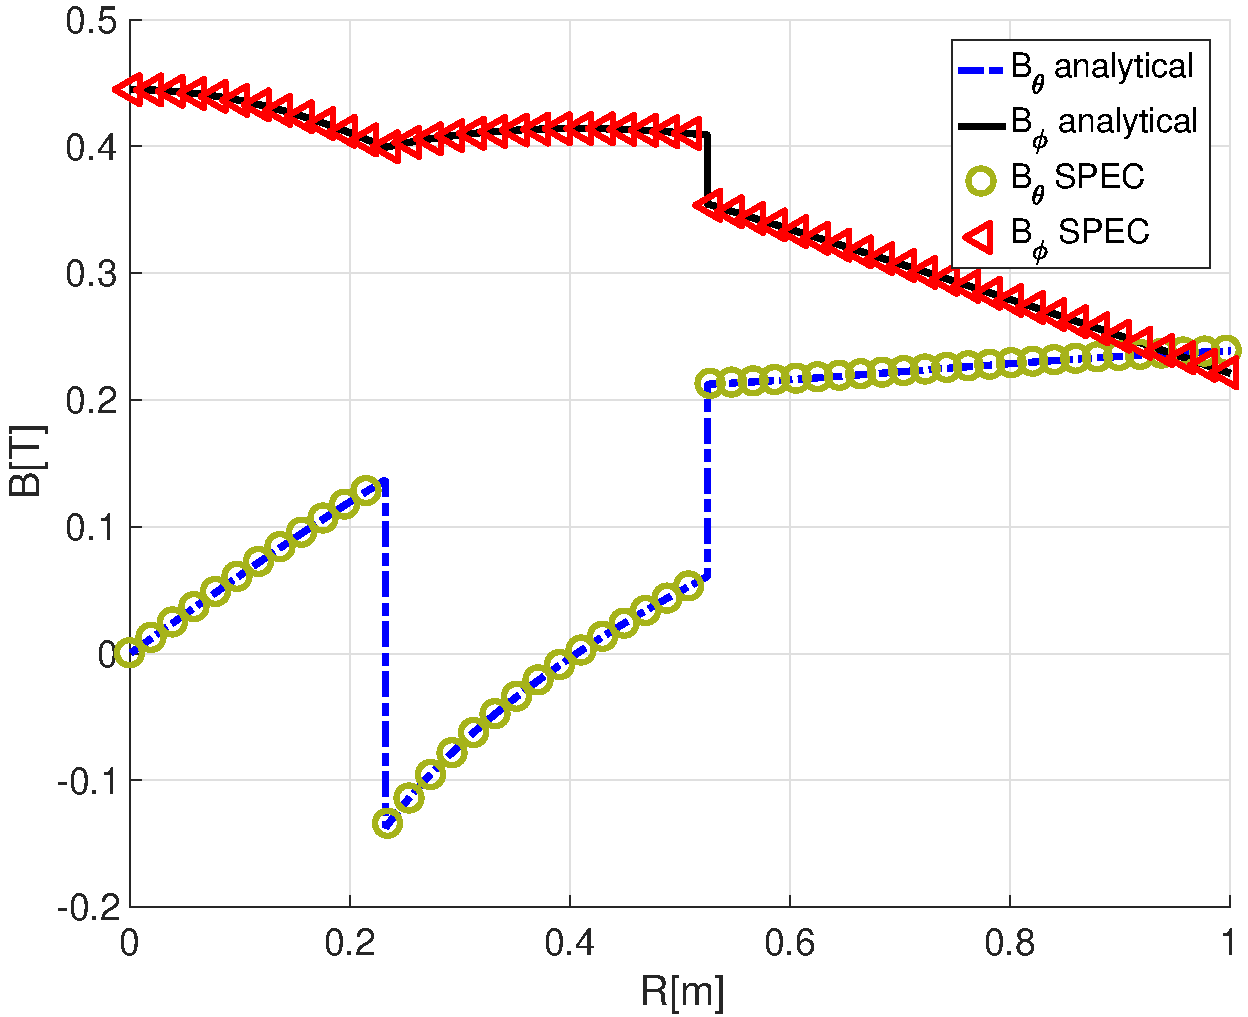
\includegraphics[width=0.5\linewidth]{main/Figures_CurrentConstraint/ABaillod_fig6.pdf}
     \caption{Magnetic field components as a function of the radius in the case of a screw pinch. Solid and dashed lines: analytical solution as given in Appendix \ref{appB}. Circles and triangles: \ac{SPEC} solution using the current constraint.}
     \label{fig:SP_constraint_verification}
 \end{figure}
 The force gradient can also be expressed in terms of Bessel functions integrals (see Appendix \ref{appB}). Figure \ref{fig:ForceGradient_Convergence_ScrewPinch} shows the normalized maximum absolute error between the force gradient obtained with \ac{SPEC} and that obtained analytically as a function of the radial resolution $L_{rad}$. As $L_{rad}$ is increased, exponential convergence is observed up until $10^{-13}$, where the error in the evaluation of the Bessel integrals starts to dominate. 
 
 \begin{figure}
     \centering
     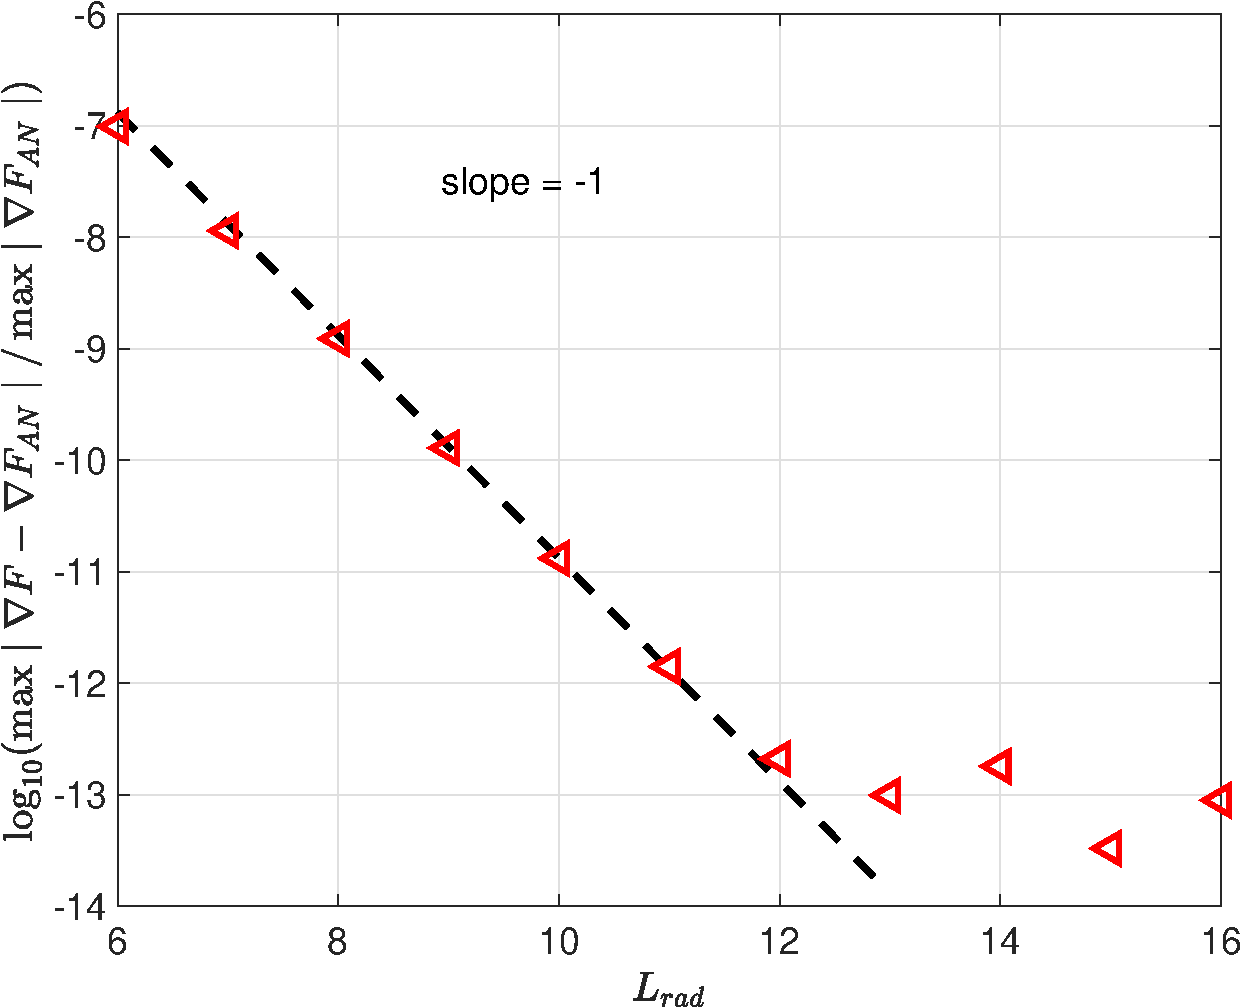
\includegraphics[width=0.5\linewidth]{main/Figures_CurrentConstraint/ABaillod_fig7.pdf}
     \caption{Semi-logarithmic plot of the maximal absolute error between the analytical force gradient, $\nabla F_{AN}$, and the force gradient obtained from \ac{SPEC}, $\nabla F$, as a function of the radial resolution for the screw pinch case.}
     \label{fig:ForceGradient_Convergence_ScrewPinch}
 \end{figure}
 
 \subsection{Verification in toroidal geometry}
 
 A verification is proposed here in the more complex case of a free-boundary, rotating ellipse (also called classical stellarator) equilibrium with $5$ field periods ($N_p=5$), multiple poloidal and toroidal modes ($M_{pol}=4$ and $N_{tor}=2$) and seven plasma volumes ($N_{vol}=7$). The pressure is set to zero and the computational boundary is defined by
 
 \begin{align}
     R &= R_{00} + R_{10} \cos\theta + R_{11}\cos(\theta - N_p\phi)\label{eq.RotEllipse_R}\\
     Z &= Z_{00} + Z_{10} \sin\theta + Z_{11}\sin(\theta - N_p\phi),\label{eq.RotEllipse_Z}
 \end{align}
 with $R_{00}=10$m, $Z_{00}=0$m, $R_{10}=-Z_{10}=1$m, $R_{11}=Z_{11}=0.25$m and $N_p = 5$ (see Figure \ref{fig:3Dplot}). We suppose here that some hypothetical coils with a total current of $\mu_0I_{coil}=42.87$Tm are able to generate a vacuum field without normal component to the computational boundary. The total toroidal magnetic flux in the plasma is set to $\psi_a=0.61\text{Tm}^2$ and the toroidal magnetic flux in the vacuum region is set to $\psi_{t,V}=1.39\text{Tm}^2$, adding up to a total toroidal magnetic flux enclosed by the computational boundary of $\psi_{t,V} + \psi_a = 2\text{Tm}^2$.
 
 \begin{figure}
     \centering
     \includegraphics[width=0.5\linewidth]{main/Figures_CurrentConstraint/ABaillod_fig8.pdf}
     \caption{\ac{3D} plot of the classical stellarator boundary as described by Eqs.(\ref{eq.RotEllipse_R})-(\ref{eq.RotEllipse_Z}). Colors indicate the magnetic field strength.}
     \label{fig:3Dplot}
 \end{figure}
  
 To the authors knowledge, no analytical solution to Eqs.(\ref{eq.BeltramiEquation}) and (\ref{eq.force_balance}) exists in this geometry. The verification is thus carried out as follows: first, a rotational transform constraint case is run with an input $\iotabar$-profile that is chosen to be $10\%$ larger than the vacuum rotational transform $\iotabar_{vac}$, \textit{i.e.} $\iotabar = 1.10\cdot\iotabar_{vac}$, so that there is a non-zero contribution from the current to the rotational transform. The volume and surface currents are evaluated from the obtained equilibrium and used to run a current constraint calculation to obtain a second equilibrium. The same initial guess for the geometry and the interfaces is used for both calculations. The rotational transform profile $\bar{\iotabar}$ is then extracted from the second equilibrium and compared to the reference $\iotabar$-profile.
 
 The vacuum rotational transform profile, as well as the profiles $\iotabar$ and $\bar{\iotabar}$ are shown in Figure \ref{fig:iota_and_current_profile} (left). The toroidal current enclosed by the plasma is mostly contained in the volumes and adds up to a total of $\sim 2.7$kA, see Figure \ref{fig:iota_and_current_profile} (right). As expected the surfaces currents $I^s_{\phi,l}$ remain small ($<10^{-2}$kA), since there are no pressure gradients to drive them. The constraint on the rotational transform $\iotabar$ is enforced on each side of the volumes' interfaces, indicated by gray dashed lines on Figure \ref{fig:iota_and_current_profile} (left). The value of $\iotabar$ at the computational boundary is not constrained. Agreement between $\iotabar$ and $\bar{\iotabar}$ up to a relative error of $\max(\mid\iotabar-\bar{\iotabar}\mid / \mid\iotabar\mid)\sim 10^{-5}$ is observed, showing that the same equilibrium can be obtained using either constraint. The maximum error between both profiles decreases as the numerical resolution is increased (data not shown).

 
 \begin{figure}
     \centering
     \hfill
     \subfloat[][]{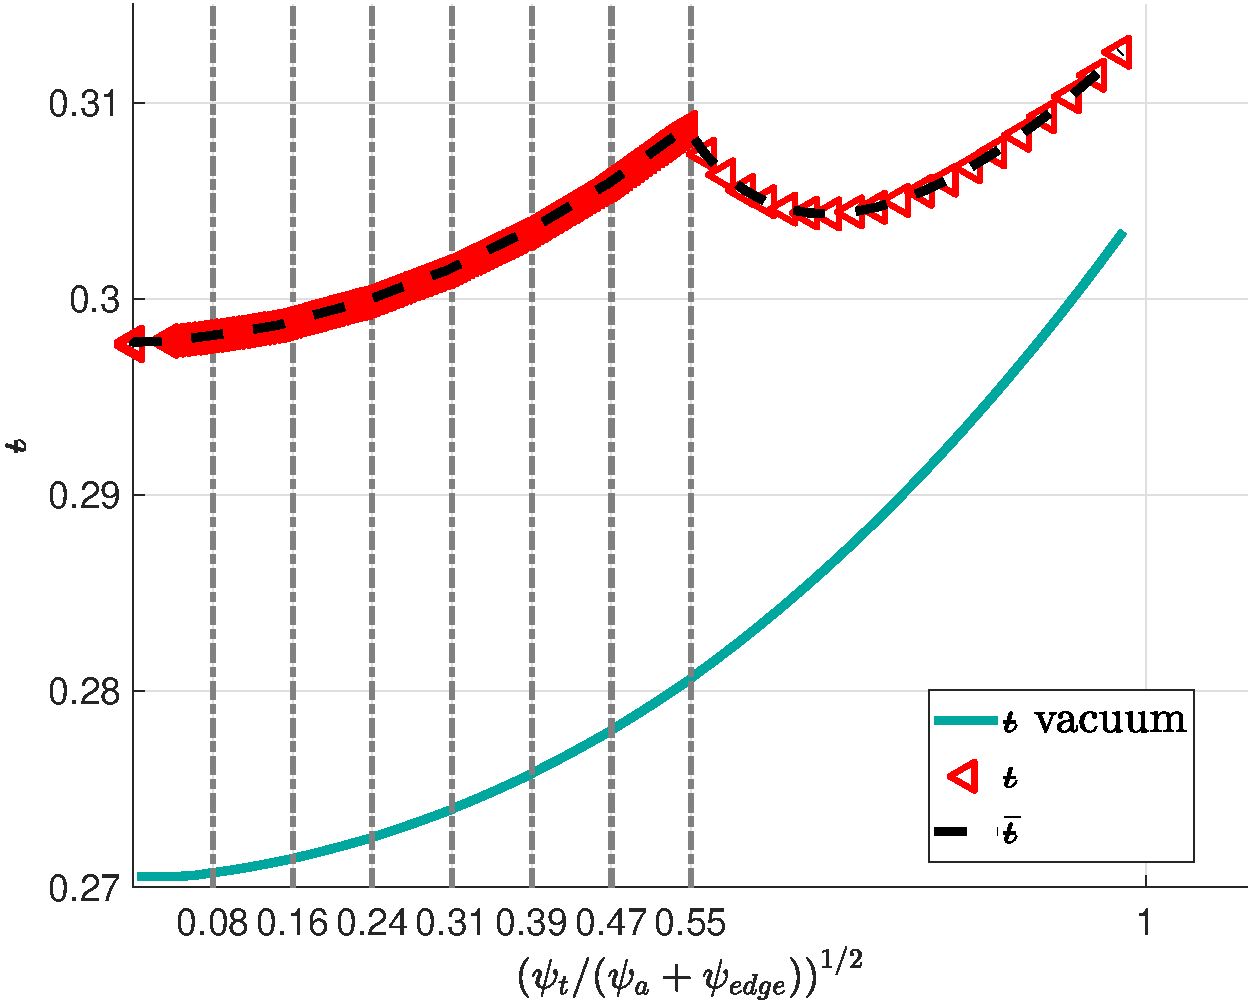
\includegraphics[width=.45\textwidth]{main/Figures_CurrentConstraint/ABaillod_fig9a.pdf}}
     \hfill
     \subfloat[][]{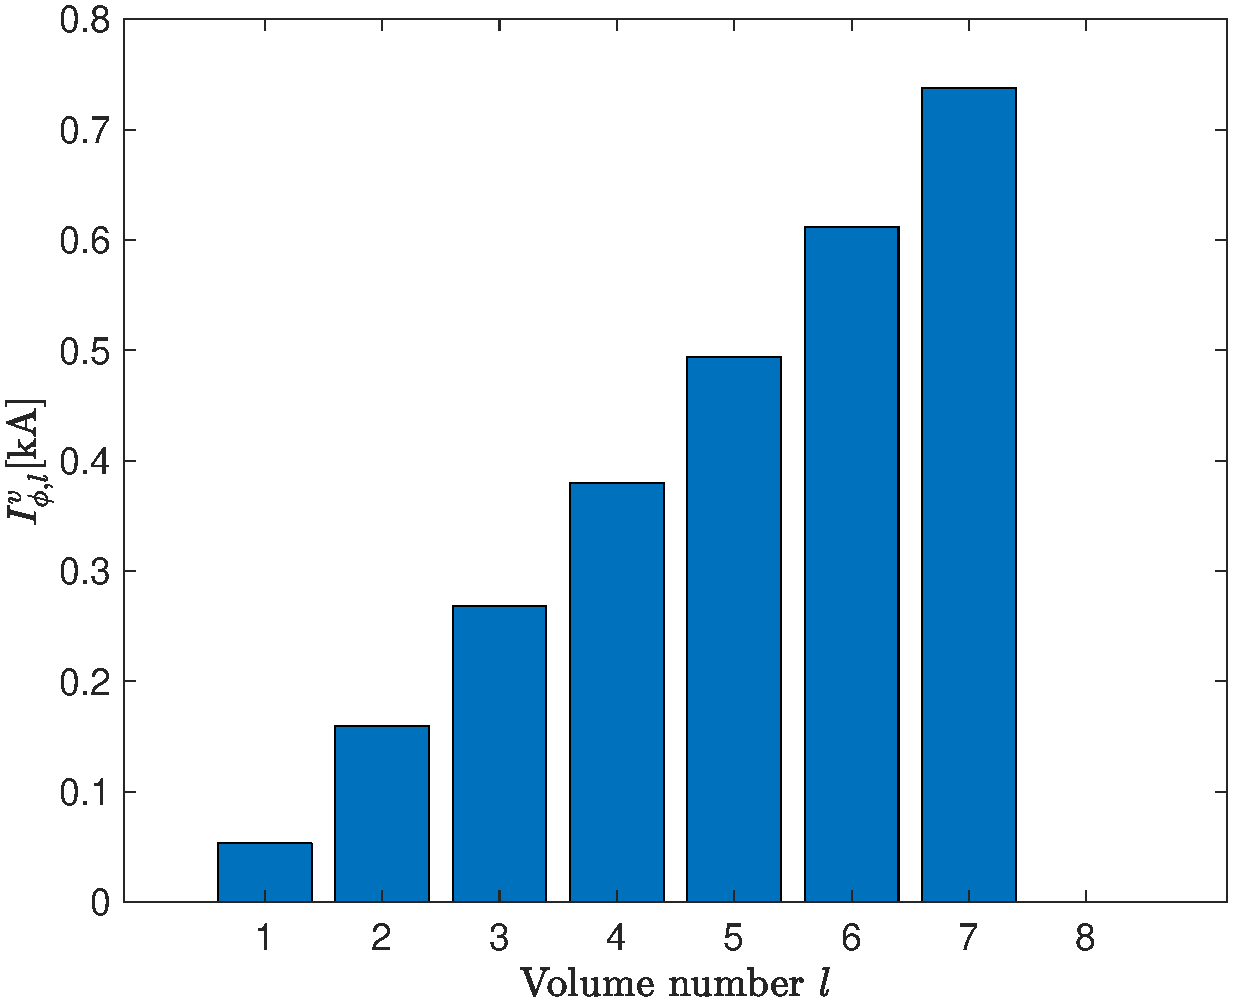
\includegraphics[width=0.45\linewidth]{main/Figures_CurrentConstraint/ABaillod_fig9b.pdf}}
     \hfill
     \caption{Left: rotational transform profile versus effective minor radius. Red triangles: $\iotabar$, input profile used in \ac{SPEC} when run at fixed rotational transform. Black, dashed line: $\bar{\iotabar}$, the output profile obtained from \ac{SPEC} when run at fixed toroidal current profile. Blue line: $\iota$-profile in vacuum. Gray dashed lines: Position of volume interfaces. Right: total toroidal current enclosed by each volume. Surface currents (not plotted), $I^s_{\phi,l}$, are smaller than $10^{-2}$[kA] and are negligible in comparison to the volume current.}
     \label{fig:iota_and_current_profile}
 \end{figure}
 
 To verify the force gradient components, we use a fourth-order centered finite difference formula \citep{Fornberg1988},
 
 \begin{equation}
     \frac{d f}{d x} = \frac{f(x-2\Delta x)  - 8f(x-\Delta x) + 8f(x+\Delta x) - f(x+2\Delta x)}{12\Delta x} + \mathcal{O}(\Delta x^4),
 \end{equation}
 to obtain $\nabla F_{FD}$, \textit{i.e.} a finite-difference estimate of the force gradient, and compare it to $\nabla F$, \textit{i.e.} the force gradient calculated in \ac{SPEC} by using analytical derivatives. The finite difference estimate is evaluated by perturbing each geometrical degree of freedom $\{x_i\}_{l=1,\ldots,N}$ by a constant value $\Delta R$. Convergence as $\Delta R\rightarrow 0$ is shown in Figure \ref{fig:conv_FG_rotell}. A convergence of order $\mathcal{O}(\Delta R^4)$ is observed down to $\sim 10^{-11}$ for $\Delta R\sim 10^{-4}$. For lower values of $\Delta R$, the finite difference approximation error is dominated by round-off error. This shows that the analytical derivatives (the force gradient) is correctly implemented in \ac{SPEC}.
 
 \begin{figure}
     \centering
     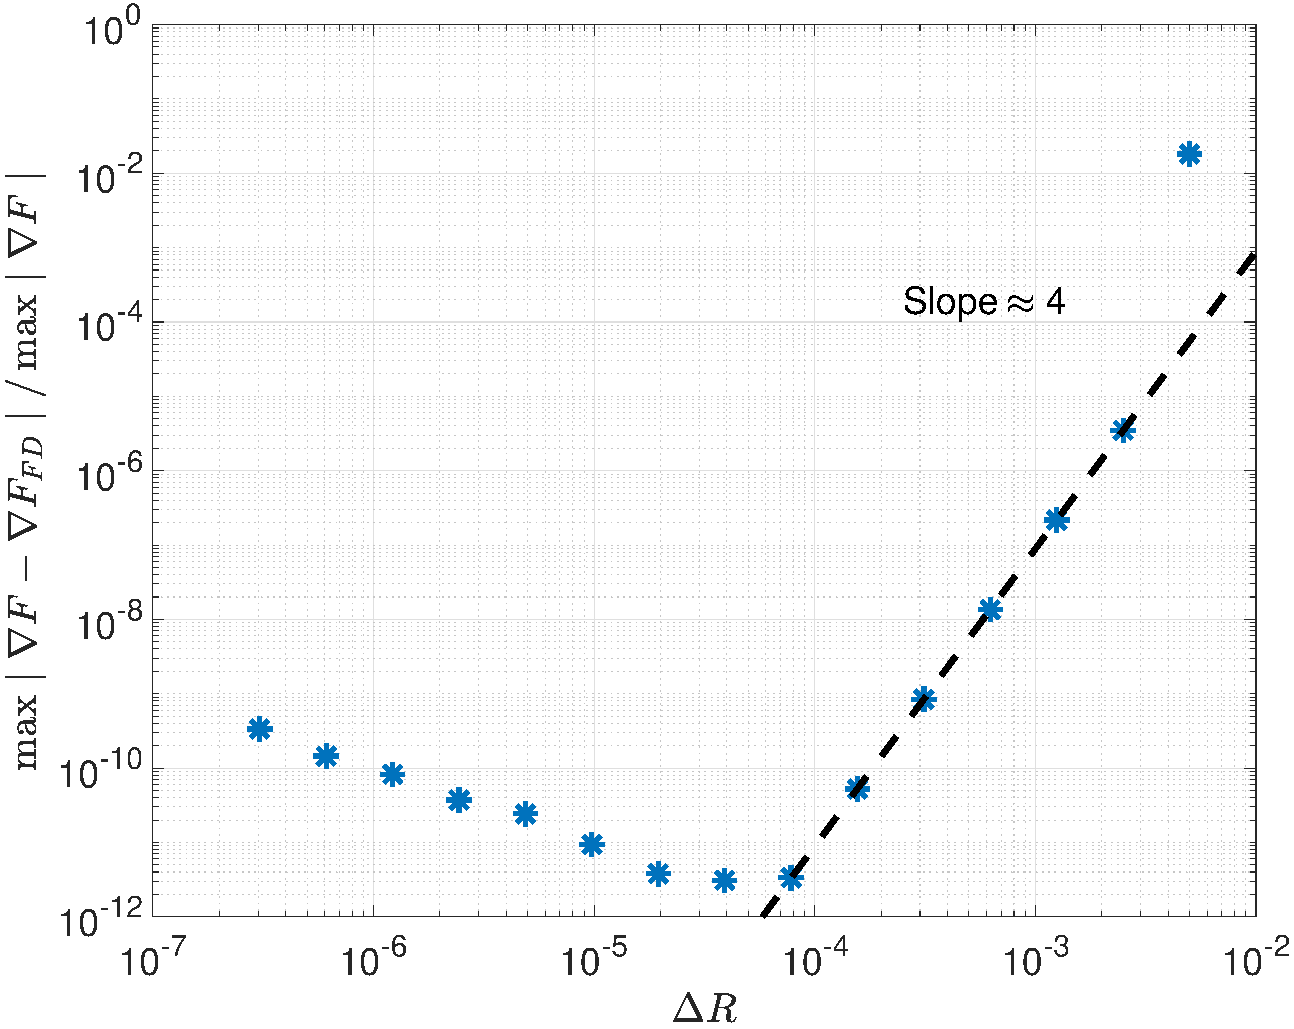
\includegraphics[width=.5\linewidth]{main/Figures_CurrentConstraint/ABaillod_fig10.pdf}
     \caption{Normalized maximum absolute error between \ac{SPEC} force gradient and a finite difference estimate in the case of a rotating ellipse. The dashed line has slope of $4$.} \label{fig:conv_FG_rotell}
 \end{figure}
 
 
 
 
 \section{Conclusion} \label{sec.discussion}
 
 Toroidal currents in \ac{MRxMHD} have been derived and expressed in terms of simple quantities. Two profiles have been identified: the volume current profile, flowing through the volumes, and the surface current profile, flowing at each volume interface. A physical interpretation has been given to each of the currents. Both profiles have been implemented as new constraints in the \ac{SPEC} code, which can now compute \ac{MRxMHD} equilibria for a given toroidal current profile. Analytical derivatives of the force on each volume interface with respect to the interfaces' geometry at fixed toroidal current have been derived and implemented in \ac{SPEC}. These derivatives speed up substantially the Newton iterations on the interface geometries.
 
 Both the new constraint and the force gradient implementation have been verified in slab, cylindrical and toroidal geometries. We presented in this paper only the latter two. In cylindrical geometry, we considered an axisymmetric screw pinch, where the obtained equilibria and force gradient could be compared to analytical solutions. In toroidal geometry, a classical stellarator geometry has been considered. The equilibrium has been verified to match the equilibrium obtained by constraining the rotational transform profile in \ac{SPEC}, and the force gradient has been compared to a finite difference estimate. 
% 
% Finally, the calculation of the ideal equilibrium $\beta$-limit in a classical stellarator with zero net toroidal current has been presented as a first application of the new \ac{SPEC} capabilities. The free-boundary calculation showed very good agreement both with a previous, simpler study \citep{Loizu2017}, and with the \ac{HBS} theory \citep{Freidberg2014, wakatani-stellarator-1998}. In the future, effects of bootstrap current on the equilibrium $\beta$-limit in a classical stellarator will be investigated. Furthermore, this new tool opens the possibility of comparing \ac{SPEC} with previous results obtained with other equilibrium codes such as PIES \citep{Drevlak2005, Hirsch2008}, and perform similar studies on present experiments such as W7-X. In particular, it is envisaged to study W7-X equilibrium $\beta$-limits and its robustness to fluctuations in the toroidal current profile.
 
% 
% \subsection{Acknowledgement}
% The authors acknowledge useful discussion with S. R. Hudson, C. Smiet, J. Schilling, J. Geiger and C. Zhu.
% 
%This work has been carried out within the framework of the EUROfusion Consortium and has received funding from the Euratom research and training program 2014 - 2018 and 2019 - 2020 under grant agreement No 633053. The views and opinions expressed herein do not necessarily reflect those of the European Commission (A.B., J.L., J.P.G.); This work is partly funded by Australian ARC projects DP170102606 (Z.Q., A.K.); This work was also supported by a grant from the Simons Foundation/SFARI (560651, AB) (A.B., J.L., Z.Q., A.K.).
%
%\subsection{Declaration of interests}
%
%The authors report no conflict of interest.

%--%--%--%--%--%--%--%--%--%--%--%--%--%--%--%--%--%--%--%--%--%--%--%--%--%--%--%--%--%--%--%--%--%--%--%







\section{Implementation of a unique angle representation \label{sec. angle representation}}

\subsection{Why a new angle representation is required}

\subscetion{The Henneberg representation}

\subscetion{Implementation}

\subsection{Discussion }


\section{Conclusion \label{sec. chap3 - conclusion}}



\end{document}